Esta estrutura de retificador utiliza uma ponte de diodos para garantir um funcionamento similar ao do retificador com ponto médio, mas sem a necessidade de uma conexão intermediária no secundário do transformador, i.e., sem a necessidade de uma fonte simétrica. Tanto o circuito quanto as etapas de funcionamento são ilustradas na figura \ref{fig:CECT}.
 
\begin{figure}[ht]
    \center
    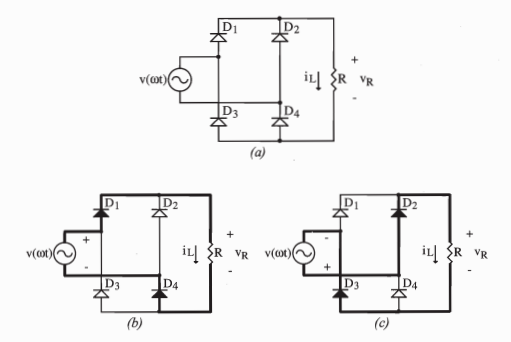
\includegraphics[scale=1]{imagens/Retif_mon_Ponte.PNG}
    \caption{(a) Circuito do retificador monofásico de onda completa em ponte com uma carga resistiva. (b) e (c) Etapas de funcionamento da ponte de diodos.}\label{fig:CECT}
    \caption*{Fonte: Eletrônica de Potência (2006)}
\end{figure}

A principal diferença é que, lidando com componentes não ideais, a presença de dois diodos em condução a todo momento implica no dobro da queda de tensão para a carga.

A tensão e a corrente aparentes à carga são idênticas as já demonstradas para o retificador de ponto médio. Seus valores médios são
\begin{align*}
    V_{L,med} &= 0,9V_o \\
    I_{L,med} &= \frac{0,9V_o}{R}
.\end{align*}

Novamente, as etapas de funcionamento apresentadas para a carga resistiva se mantém para uma carga indutiva. O comportamento também se mantém idêntico ao caso do ponto médio.

A presença de um transformador pode ser analisada de forma similar ao caso do retificador de meia onda, uma vez que o secundário não mais precisa ter uma conexão intermediária como no caso do retificador com ponto médio. Tal circuito é ilustrado na figura \ref{fig:RPAT}.

\begin{figure}[ht]
    \center
    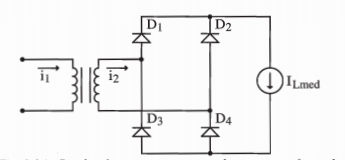
\includegraphics[scale=1]{imagens/RetPontTransf.PNG}
    \caption{Retificador em ponte alimentado por um transformador.}\label{fig:RPAT}
    \caption*{Fonte: Eletrônica de Potência (2006)}
\end{figure}

A corrente eficaz no secundário é 
\begin{align*}
    I_{2,ef} &= \sqrt{ \frac{1}{2\pi} \int_0^{2\pi} I_{L,med}^2 d(\omega{t}) } \\
	      &= I_{L,med}
,\end{align*}
enquanto a tensão é \[
V_{2,ef} = \frac{V_{L,med}}{0,9}
.\] 

Dessa forma, podemos determinar a potência aparente do transformador \[
    S_2 = V_{2,ef}{I_{2,ef}} = \frac{V_{L,med} {I_{L,med}}}{0,9}
,\] sendo $P_{L} = V_{L,med}I_{L,med}$, portanto \[
    S_2 = 1,11 P_L
.\] 

Vemos que o retificador em ponte aproveita melhor o enrolamento do secundário do transformador do que o retificador de ponto médio.

Esses retificadores normalmente são utilizados na alimentação de circuitos eletrônicos mais comuns (e.g., eletrodomésticos, computadores), no carregamento de baterias e na alimentação de enrolamentos de campo de máquinas elétricas. 

